%!TEX root = ../main.tex
\section{Symphony: Data Discovery over Multimodal Data Lakes}
\label{sec:learning}

\begin{figure}[b!]
\begin{center}
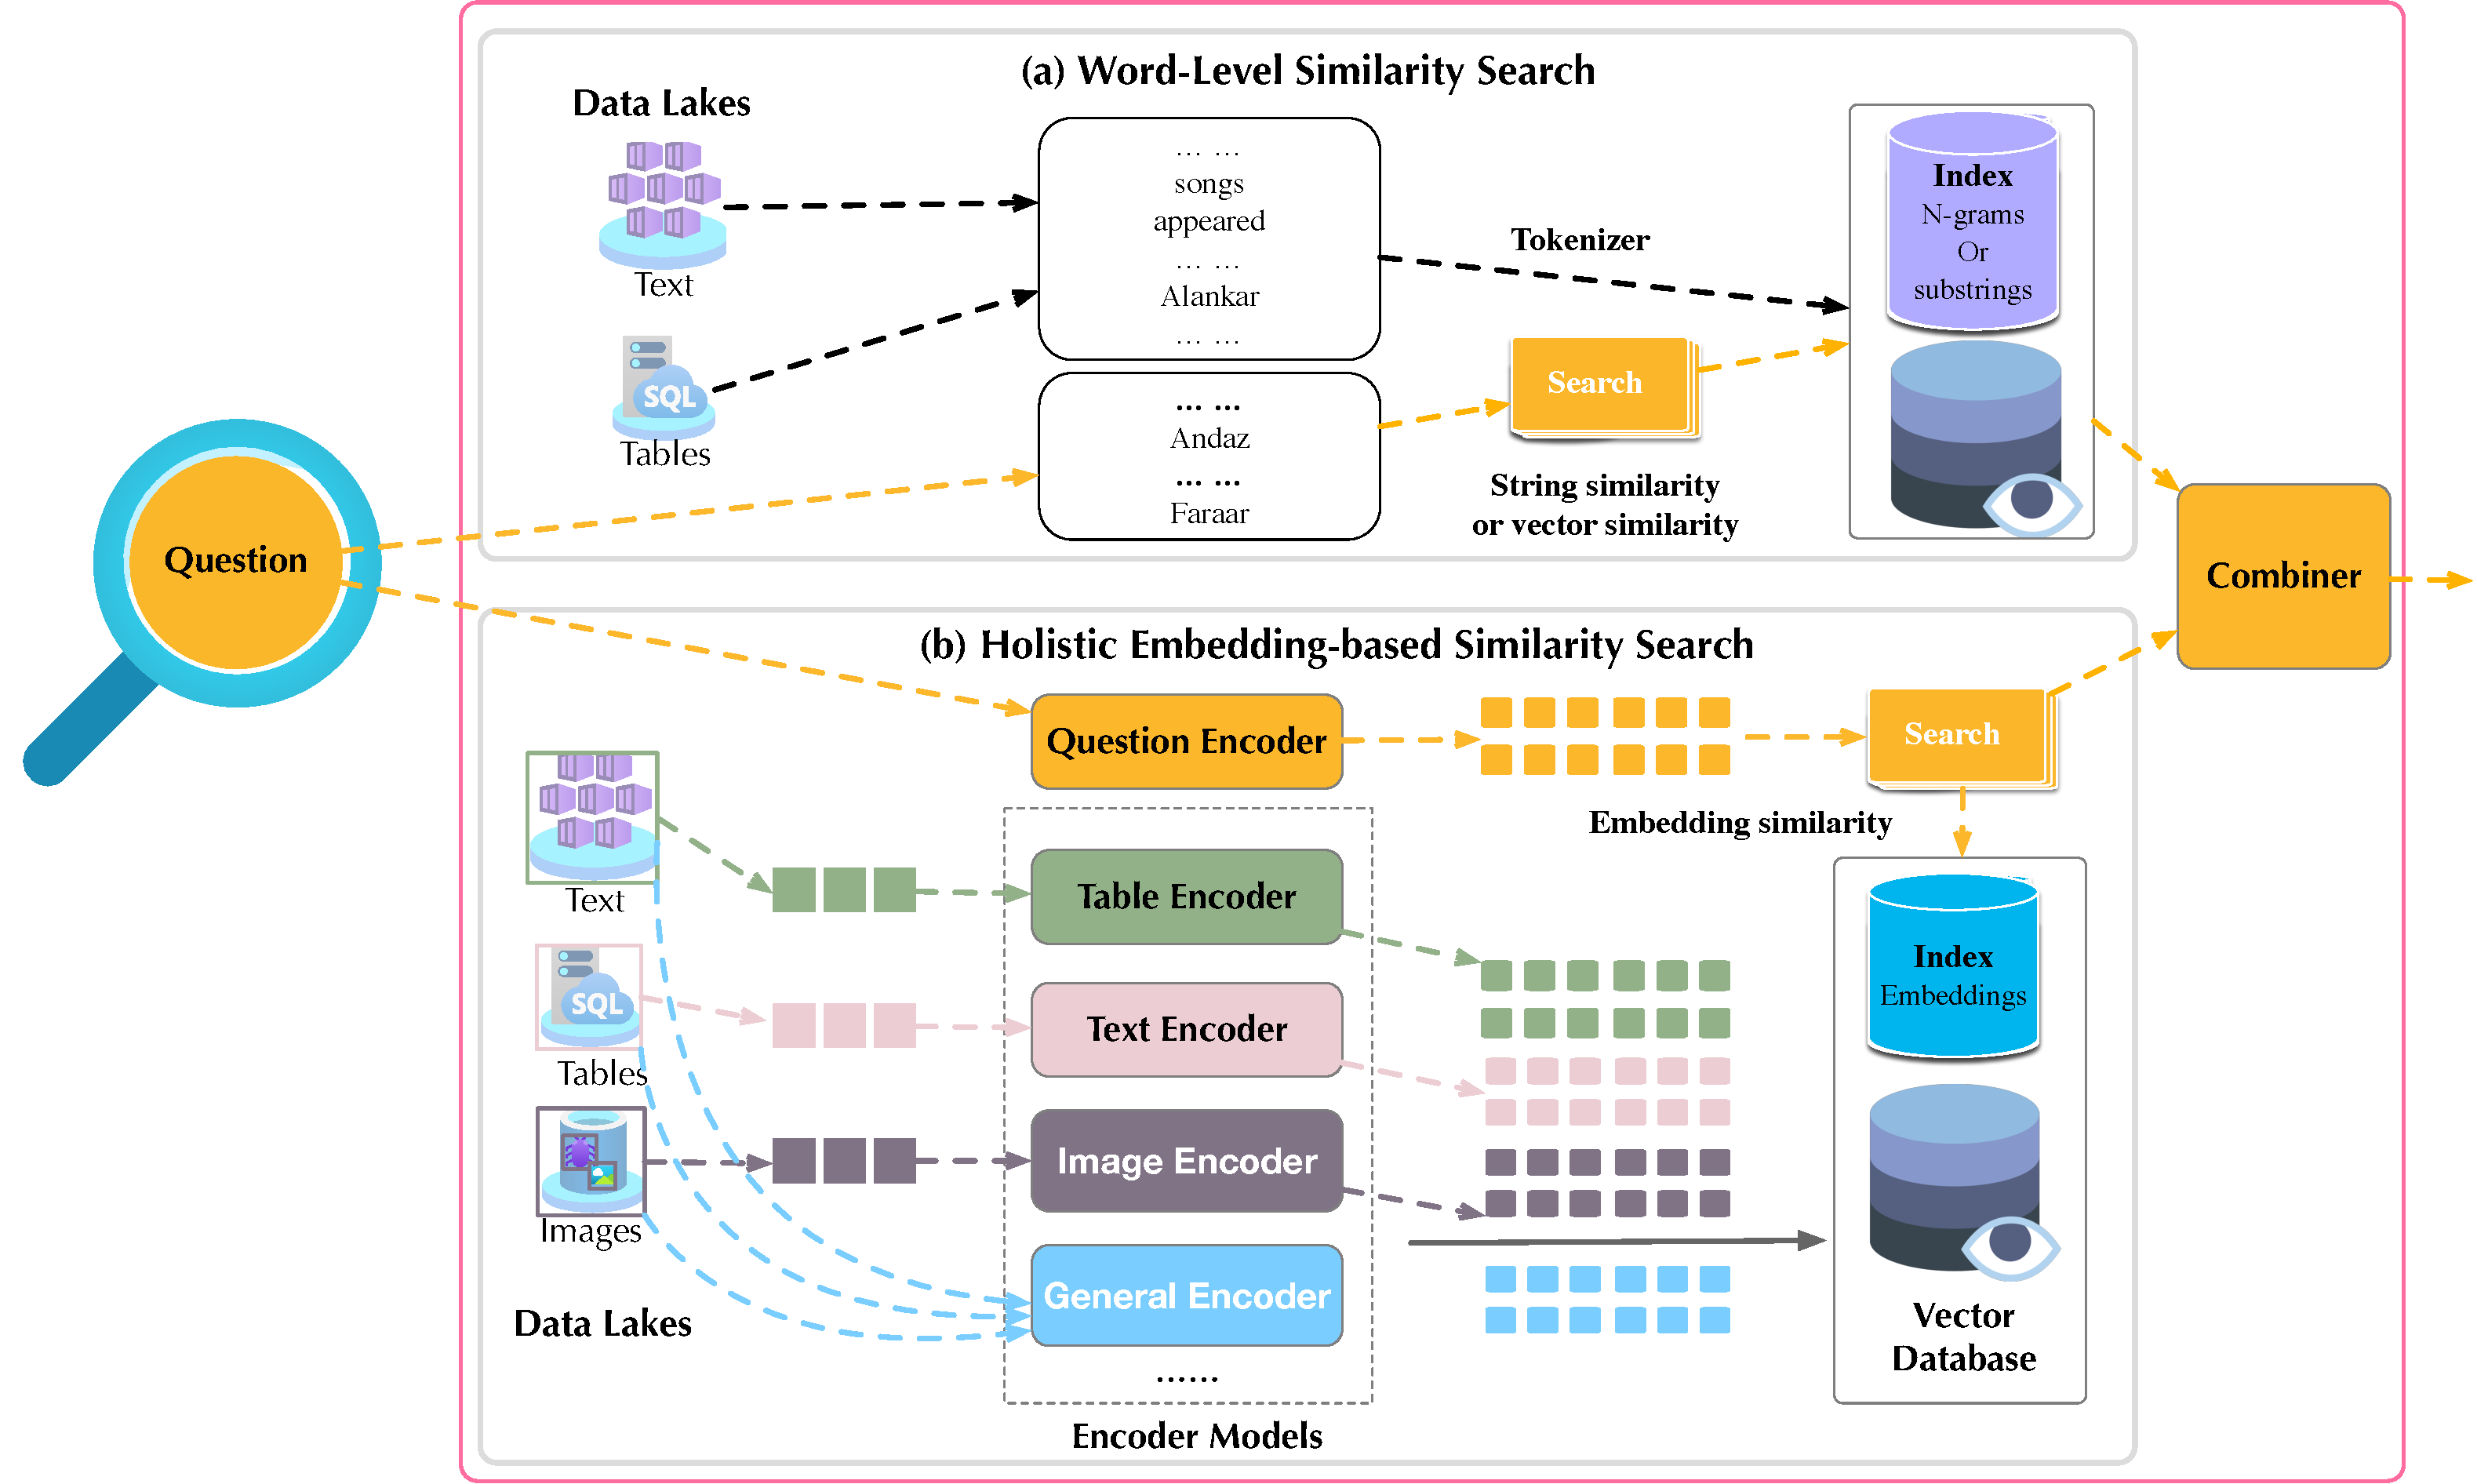
\includegraphics[width=0.9\textwidth]{submissions/Nan2024/figs/discovery.pdf}
\vspace{-1em}
\caption{The \discovery Module.}
\label{fig:discovery}
\end{center}
\end{figure}

% The core of supporting retrieval across diverse data types is the representation learning of different modalities, \ie how to encode different modalities into meaningful representations.

%\subsection{Overview of Data Discovery}

Data discovery is the process of identifying relevant data files from multimodal data lakes efficiently. As shown in Figure~\ref{fig:discovery}, \sys provides two main categories of data discovery methods: 
(a) word-level similarity search and 
(b) holistic embedding-based similarity search. These methods are chosen based on a balance between efficiency and effectiveness, enabling retrieval of relevant data from data lakes, thus supporting both reasoning and verification.

\stitle{Word-level similarity search} breaks down queries and data items in the data lakes into words (or terms), retrieves and ranks data items based on combined word-level similarity, as shown in Figure~\ref{fig:discovery} (a). Methods like BM25, TF-IDF, and Jaccard similarity are used. These approaches are simple, interpretable, and computationally efficient, making them ideal for scenarios with high word overlap between the query and data items.

\stitle{Embedding-based similarity search} encodes multimodal data items and queries into high-dimensional vectors in a shared embedding space, enabling fast and precise similarity calculations. As shown in Figure~\ref{fig:discovery}, in this process, multimodal data (\eg text, tables or images) are encoded into dense vector embeddings. These embeddings are then stored in a vector database (\eg Meta Faiss), and indexed for fast similarity-based retrieval, typically using efficient distance metrics like cosine similarity or dot product.
%
To support various data representations, \sys investigates the following two encoding strategies:

\be
	\itemsep-1mm 
	\item \textbf{\textit{Modal-specific Representation Learning.}} 
	This strategy uses models tailored to each data type (\eg text encoder~\cite{karpukhin-etal-2020-dense}, table encoder~\cite{rpt} or image encoder CLIP~\cite{radford2021learning}), capturing unique features like intricate table structures or text nuances, making it ideal for precise retrieval within individual modalities. %While text and image representation is well-studied, we leverage existing developed models: DPR~\cite{karpukhin-etal-2020-dense} for text and . However, table representation remains underexplored, presenting unique challenges due to its inherent structural complexity and diversity in data formats. (Section~\ref{subsec:table_rep})

	\item \textbf{\textit{Modal-agnostic (Cross-Modal) Representation Learning.}} 
	This strategy learns a shared embedding space, using a General Encoder, through cross-modal representation learning (see \cite{symphony} for more details), enabling similarity comparisons across modalities. This approach supports queries that can retrieve relevant items from different modalities, enhancing interoperability where cross-modal relationships are crucial. %(Section~\ref{subsec:multimodal_rep})
\ee

% \textbf{(2) Modal-specific Representation} uses models tailored to each data type (\eg text, tables, images), capturing unique features like intricate table structures or text nuances, making it ideal for precise retrieval within individual modalities. While text and image representation is well-studied, we leverage existing developed models: DPR~\cite{karpukhin-etal-2020-dense} for text, CLIP~\cite{radford2021learning} and DeepFace~\cite{deepface} for images. 
% For image representation, in particular, we go further by constructing a relational graph that captures the relationships between individuals in images, providing a structured way to model interactions. \yang{modify this to align with your content.}
% For table representation, it remains underexplored, presenting unique challenges due to its inherent structural complexity and diversity in data formats. Our attempts in this area are further discussed in Section~\ref{subsec:table_rep}.

% \sys further refines the results of embedding-based similarity search by incorporating a \textbf{human-in-the-loop selection} mechanism. This step allows human reviewers to evaluate and select the most relevant items among the top candidate results, providing valuable feedback that enhances the accuracy of cross-modal similarity scoring. By incorporating these annotations, \sys can gradually improve its retrieval alignment with human expectations and explore few-shot meta-scoring models to automate future scoring tasks with minimal human intervention.



% \begin{figure}[t!]
% \vspace{-2em}
% \begin{center}
% 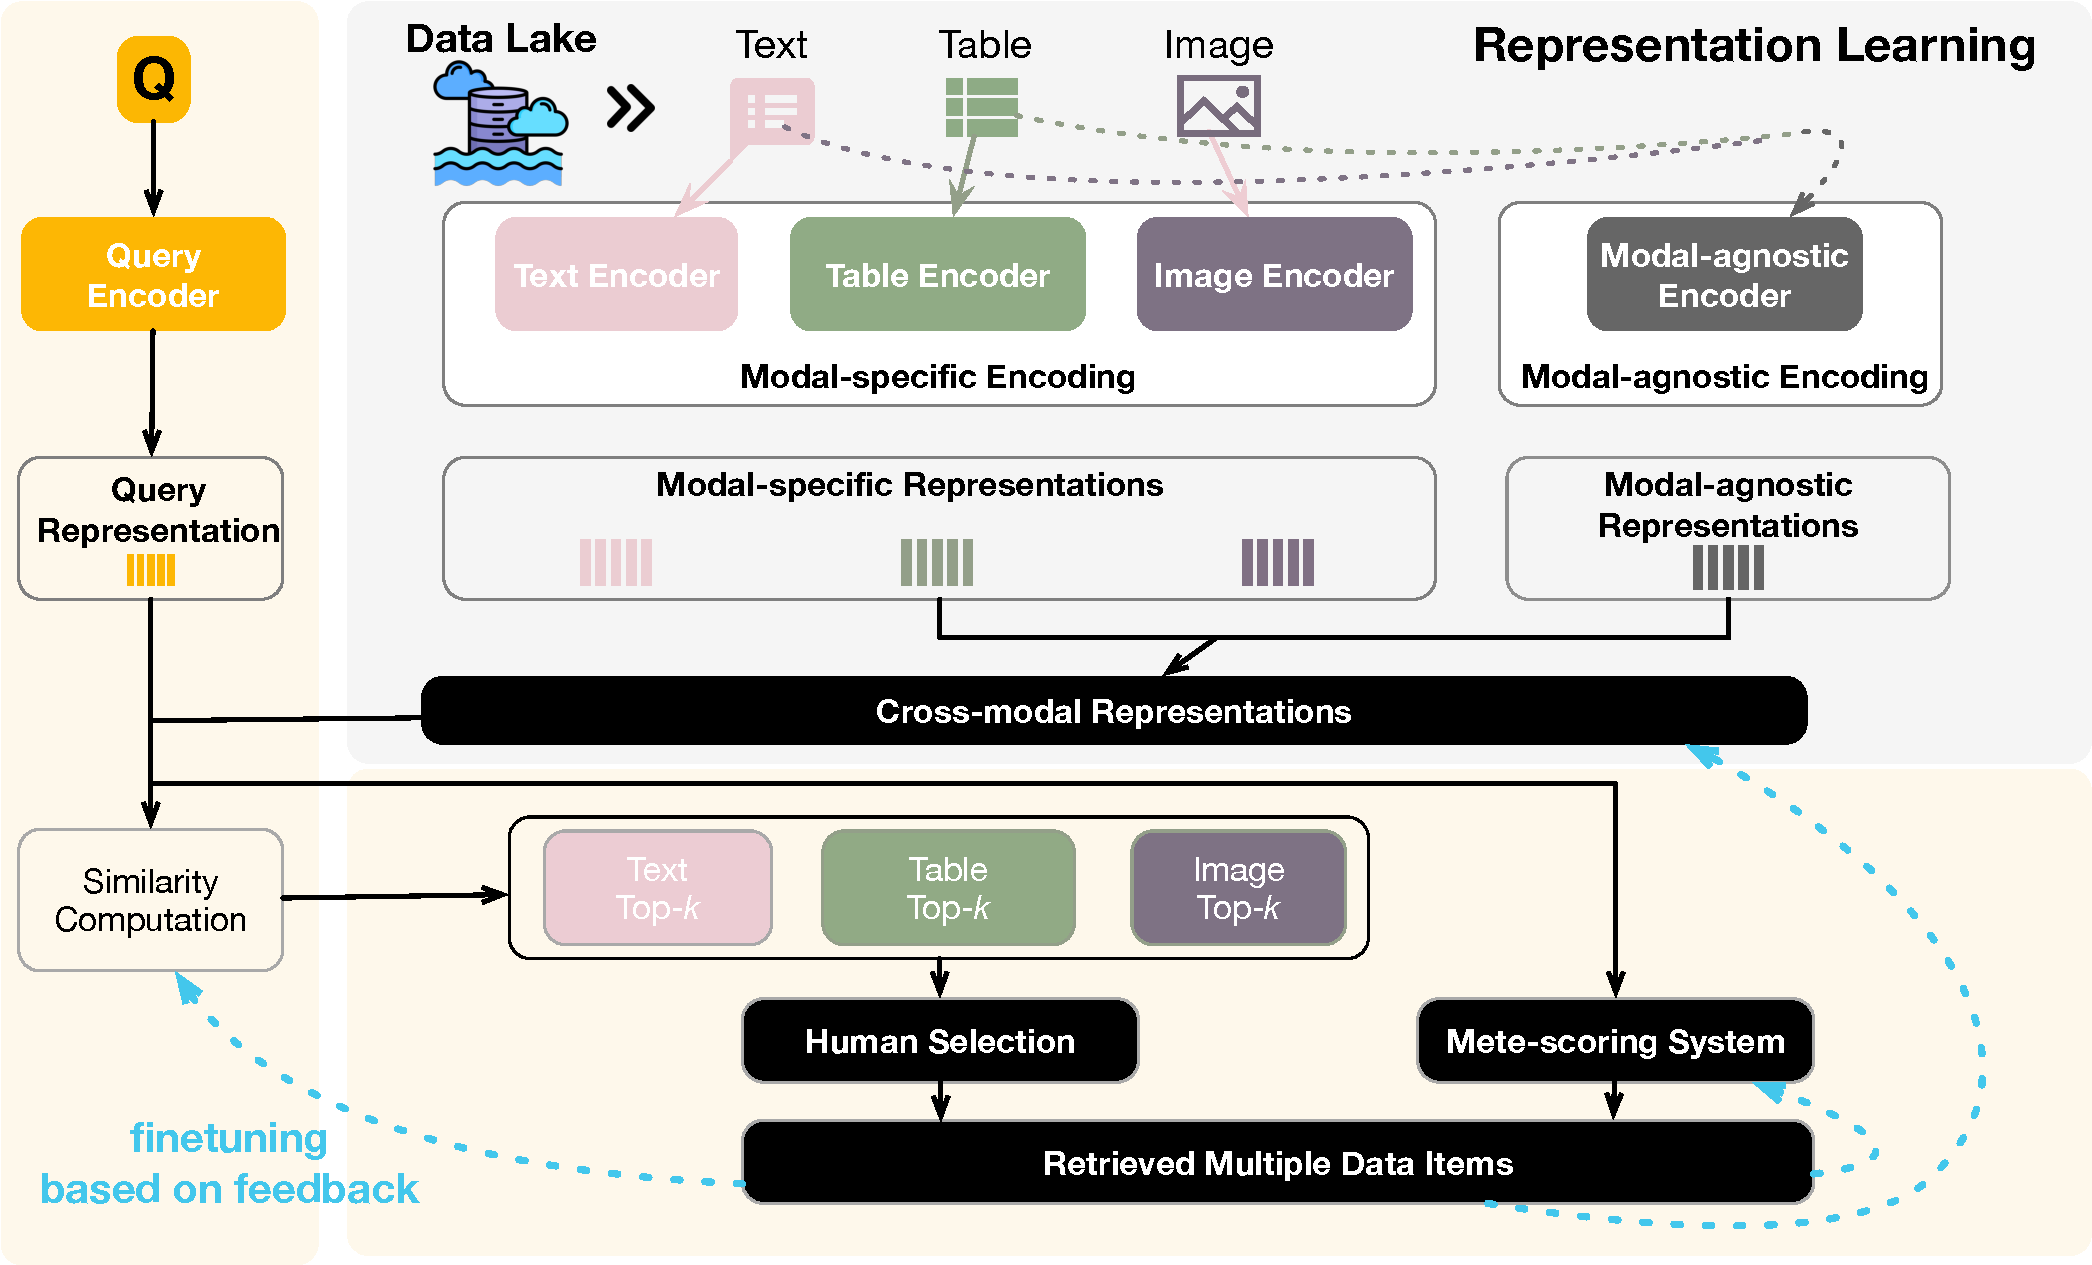
\includegraphics[width=0.9\textwidth]{submissions/Nan2024/figs/rep.pdf}
% \vspace{-1em}
% \caption{Representation Learning in \sys.}
% \label{fig:rep}
% \end{center}
% \vspace{-2em}
% \end{figure}


% \subsection{Modal-Agnostic Representation Learning}
% \label{subsec:multimodal_rep}

% In \sys, modality-agnostic (cross-modal) representation learning encodes multimodal items within a unified, high-dimensional embedding space, allowing for seamless retrieval across diverse data types. To standardize inputs across different modalities, \sys initially converts each data item into a compatible sequence format. Text data is directly tokenized, while structured data, such as tables, is serialized into linear sequences. For instance, tables are represented as linearized sequences of rows and columns, as shown with Table T1 in Figure~\ref{fig:reasoning}: \texttt{Year | Song | Film | ... || 1971 | Zindagi Ek Safar | ...}. Such serialized representations enable consistent application of language modeling techniques across modalities.


% For pre-training methods, traditional ones face limitations: (1) they often produce token-level embeddings, which are aggregated into sequence-level embeddings that do not effectively capture the entirety of the input; (2) they tend to produce embeddings tightly coupled with specific query types, limiting their generalization ability. 
% % This results in representations that may not generalize well to new queries or modalities, as they can fail to capture all the critical information. 
% To address these issues, \sys employs \textbf{Self-supervised Information Compression} to learn query-agnostic representations that capture essential information across different modalities. The key idea is to pre-train an AutoEncoder-based model that creates fixed-size embeddings. The AutoEncoder consists of an encoder that compresses the input data into a fixed-size embedding, and a decoder that reconstructs the original input from the embedding. By training the model to minimize the reconstruction error, the encoder learns to capture the most vital features of the input data in the fixed-size embedding. This strategy leverages the information compression ability of AutoEncoder, while still preserving the power of the Transformer architecture.  After pre-training, \sys uses the encoder as a general-purpose cross-modal representation model for efficient retrieval.

% To maintain generality across diverse queries and avoid modality-specific limitations, \sys employs Self-supervised Information Compression. This technique produces embeddings that capture essential information without being overly influenced by specific query types. Instead of relying on task-specific features, \sys pre-trains an AutoEncoder-based model to create fixed-size embeddings, which are capable of reconstructing the original input data. The encoder-decoder structure allows the encoder to compress vital features, ensuring that the embeddings retain a comprehensive representation of each data item. After pre-training, the encoder functions as the cross-modal representation model, which is both query-agnostic and efficient for scalable retrieval.


%%%%%%%%%%%%%%%%%%%%%%%%%%%%%%%%%%%%%%%%%%%%%%%%%%%%%%%%%%%%
% \subsection{Modal-Specific Representation}
% \label{subsec:modal_specific}
%%%%%%%%%%%%%%%%%%%%%%%%%%%%%%%%%%%%%%%%%%%%%%%%%%%%%%%%%%%%

% \stitle{Image Representation Learning}
% \zzx{To support image-image and text-image retrieval, we use CLIP~\cite{radford2021learning} to extract features from images, encoding each image \( I \) as a feature vector \( V \). For entity-level, fine-grained queries that require more specific image regions, we also use DeepFace~\cite{deepface} to extract and encode faces within the image as vectors \( V_f \).}

% \subsection{Image Representation Learning}
% \label{subsec:image_rep}


% \subsection{Table Representation Learning}
% \label{subsec:table_rep}

% \begin{figure}[t!]
% \vspace{-2em}
% \begin{center}
% 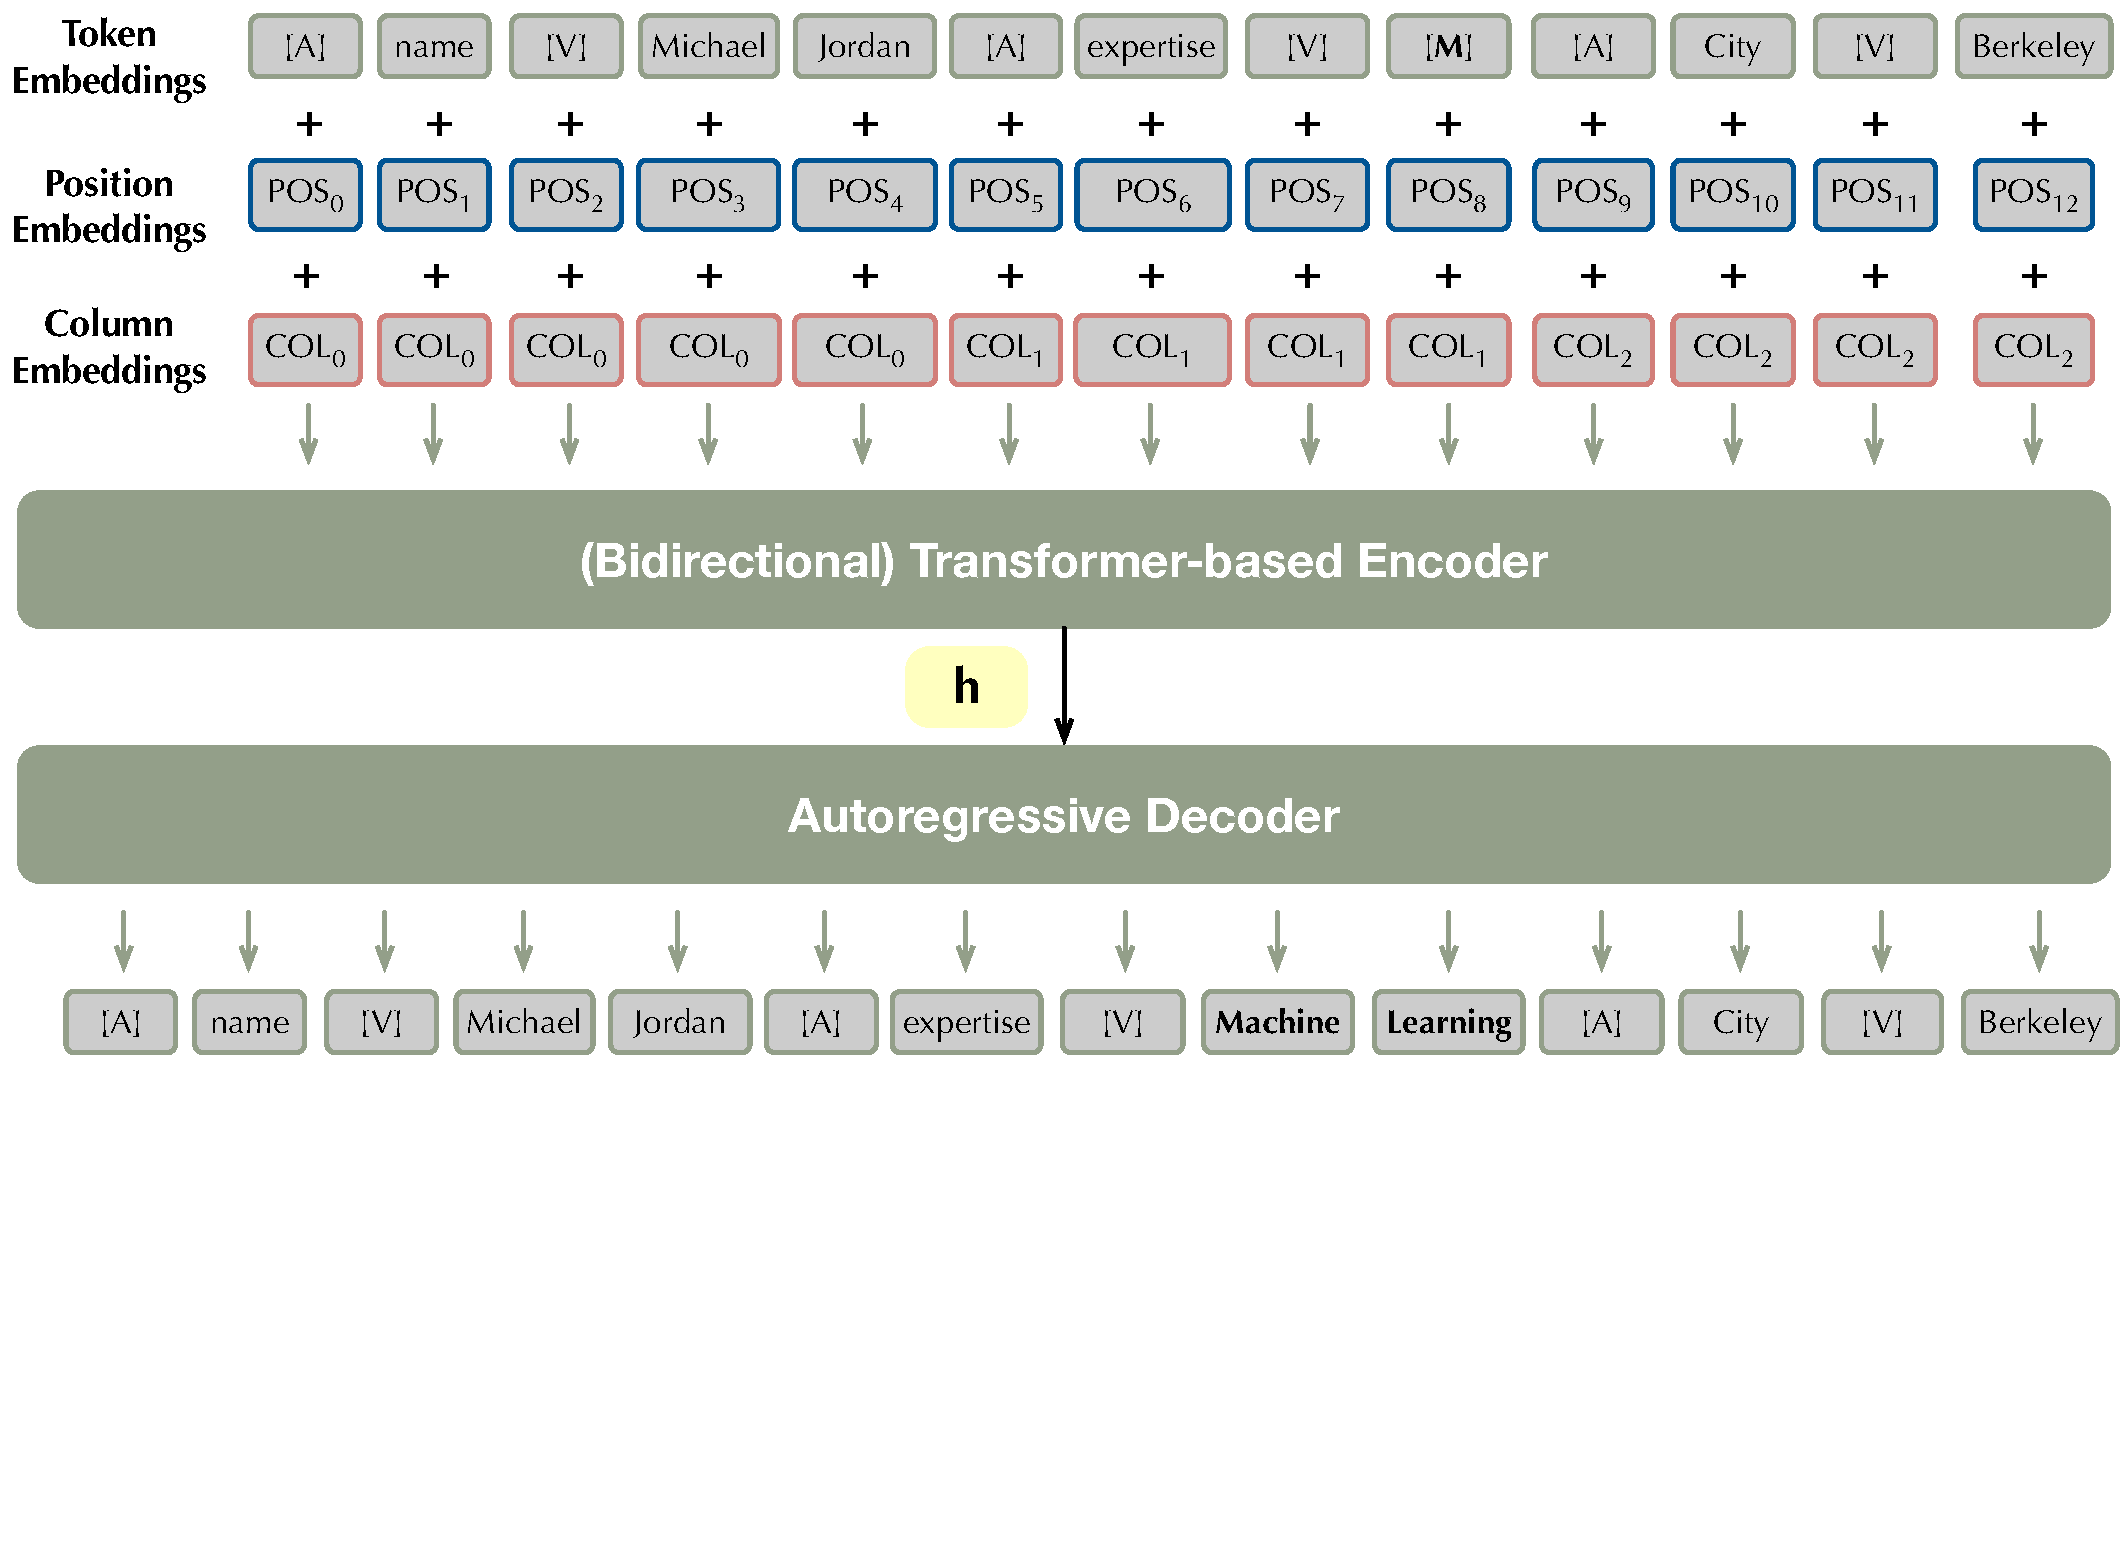
\includegraphics[width=0.8\textwidth]{submissions/Nan2024/figs/table_learning.pdf}
% \vspace{-1em}
% \caption{RPT~\cite{rpt}: Table Representation Learning.}
% \label{fig:tab_rep}
% \end{center}
% \vspace{-2em}
% \end{figure}


% Within modal-specific representation, we focus our attention on the less-explored area of table representation learning, which remains challenging and less developed compared to text representation. Unlike text, tables follow a structured format, which requires specialized techniques for learning effective representations. Here, we present our attempt to capture and embed essential information from tables, known as Relational Pretrained Transformers (RPT)~\cite{rpt}.

% Our primary objective with RPT is to learn a comprehensive and context-aware representation for relational tables that can be directly applied to tasks such as data discovery. Given that tables are structured around tuples, \ie each tuple encapsulates a complete and semantically coherent record, tuple-level learning becomes critical, as it allows the model to grasp the core relational structure inherent to tables. Thus, we designed \textbf{tuple-to-tuple pretraining}, which takes an incomplete tuple as input and outputs the reconstructed one, to enable the model to fully understand and embed the relationships within each tuple. Next, we will discuss how RPT implements tuple-to-tuple pretraining through its model design, input processing, and training task.

% \stitle{Model Architecture.}
% As shown in Figure~\ref{fig:tab_rep}, we adopt a standard sequence-to-sequence (encoder-decoder) Transformer model, following the structure of BART~\cite{DBLP:conf/acl/PressSL20}. The encoder processes the input corrupted tuple using a bidirectional approach, enabling it to capture contextual dependencies across the entire tuple. It generates an intermediate representation $h$, which contains the learned relationships within the tuple. 
% This representation is then passed to a left-to-right autoregressive decoder, which reconstructs and completes the tuple by generating all tokens sequentially. 

% \stitle{Input Processing.}
% RPT takes a tuple as input, treating it as a structured sequence of attribute-value pairs to capture the table’s relational structure. To distinguish attributes from values and enhance tuple-level semantics, we introduce special tokens 
% [\textbf{A}] and [\textbf{V}]. Each attribute name is prefixed with [\textbf{A}] (\eg [\textbf{A}] name), and each attribute value is prefixed with [\textbf{V}] (\eg [\textbf{V}] Michael Jordan), creating a clearer structure.
% %
% Further, RPT incorporates positional and column embeddings to enrich the input with table-aware metadata. Positional embeddings mark each token's position in the sequence, while column embeddings provide information about each token’s originating column. For instance, in a tuple, ``name'' may have a positional embedding POS$_1$ and a column embedding COL$_0$. These embeddings allow RPT to process tuples with greater context sensitivity, preserving relational semantics within the table structure.

% \stitle{Unsupervised Pretraining.}
% For unsupervised pretraining on tables, the model is trained to reconstruct entire tuples from corrupted ones, optimizing a reconstruction loss by minimizing the cross-entropy between the model's output and the masked original value.

% To achieve effective pretraining, we use two types of MLM tasks:
% (1) Token Masking: Individual tokens within an attribute value are replaced with [\textbf{M}] (\eg masking ``Michael'' in ``Michael Jordan'' with [\textbf{M}]), while attribute names (\eg ``[\textbf{A}] {name}'') are not masked.
% (2) Attribute Value Masking: Entire attribute values (\eg ``Michael Jordan'') are masked out by a single token [\textbf{M}].
% These tasks help the model capture token-level and cell-level understanding within tuples while also capturing the holistic meaning of the tuple. By training the model to reconstruct complete tuples rather than just individual masked tokens, we encourage the intermediate representation to compress the full semantic content of the tuple. After pretraining, we keep the encoder and use its intermediate representation $h$ as the tuple's final representation.

% % \begin{itemize}
% %     \item Core Idea: developing representations that can handle the unique characteristics of relational tables, such as mixed data types and unordered attribute sets, thus enabling these models to perform various data preparation tasks by reasoning over relationships within tabular data.
% %     \item Input: Serialized Tuple
% %     \item Model Architecture: Transformer (BART?)
% %     \item Training Task: MLM allows to train a model by masking out token(s) and forces the model to predict the missing token(s), which has proved effective by BERT on many NLP tasks. MLM can be used to mask (partial) attribute values for self-learning on tables.
% %     \item In reference, take the mean-pooled representation generated from the encoder.
% % \end{itemize}

% \stitle{Discussion about more recent methods.}
% Recently, dense retrieval has gained prominence as an effective approach in table representation learning. Unlike approaches that use a single transformer encoder, dense retrieval~\cite{herzig-etal-2021-open} leverages separate encoders for both the question and the table, applying contrastive learning to align question embeddings closely with relevant table embeddings while distancing them from irrelevant ones. This contrastive objective aligns well with data discovery goals, enhancing retrieval accuracy by emphasizing semantic relationships between questions and tables.

